\documentclass{report}
\usepackage[pdftex,hyperindex,unicode]{hyperref}
% define the title
% Text layout
%\topmargin 0.0cm
%\oddsidemargin 0.5cm
%\evensidemargin 0.5cm
%\textwidth 16cm
%\textheight 21cm

\usepackage{graphicx}

% Support cyrillic
\usepackage[utf8]{inputenc}
\usepackage[russian]{babel}

% Inkscape generated tex uses color.sty
\usepackage{color}
\graphicspath{{figs/}}
% Make inkscape regenerate image if .svg file is newer
% than .pdf
% http://mirrors.ctan.org/info/svg-inkscape/InkscapePDFLaTeX.pdf
\newcommand{\executeiffilenewer}[3]{%
  \ifnum\pdfstrcmp{\pdffilemoddate{#1}}%
  {\pdffilemoddate{#2}} > 0 {\immediate\write18{#3}}\fi}
\newcommand{\includesvg}[1]{%
  \executeiffilenewer{#1.svg}{#1.pdf}%
  {inkscape -z -D --file=#1.svg %
   --export-pdf=#1.pdf --export-latex}%
  \input{#1.pdf_tex}%
}

% Start new page with each section
% http://tex.stackexchange.com/questions/9497/start-new-page-with-each-section
\usepackage{titlesec}
%\newcommand{\sectionbreak}{\clearpage}

% Add Bibliography to the Table of Contents as an unnumbered item
\usepackage[nottoc,notlot,notlof]{tocbibind}


\begin{document}
\author{Anna Tikhonova}
\title{Static Analysis of Behavioural Properties of Stream Synchronisers}
\date{\today}
% generates the title
\maketitle
% insert the table of contents
\tableofcontents
%\begin{abstract}
% The abstract abstract.
%\end{abstract}


% Chapters.
%Kahn's fixed-point semantics:
%A network of continous functions is continous
\chapter{Related Work}\label{chap_found}
In this chapter we provide relevant theoretical background in coordination programming and stream processing. We pick a recent component-system example from each field. Then, we describe the combined approach to coordination programming and stream processing, implemented in\added{ \ak\ predecessor} \textsc{S-Net}\deleted{ and \ak\, and explain the concepts behind \ak\ in more detail}. We sum up the chapter with a comparison of the \replaced{three}{four} components systems, including their approaches to synchronisation.


%Approaches to synchronisation.
%Synchronisation facilities in coordination languages.
    \section{Coordination Programming}
The coordination paradigm offers a promising way to address some issues related to the development of efficient parallel systems. Programming a parallel system can be seen as a combination of two activities: the actual computing part comprising a number of processes that manipulate data and a coordination part that is responsible for communication between the processes.

In the main, coordination is managing dependencies between components. Since the computation is completely separated from the coordination, the processes that comprise the former are seen as black boxes. The programming languages used to write the computational code do not play an important role in setting up the coordination scheme.

Existing coordination models\footnote{A coordination model encompasses entities being coordinated, a means of coordination and a semantic framework} are described in details in the survey \cite{papadopoulos} by G. Papadopoulos and F. Arbab. They argue that these models fall into two major categories of coordination programming, namely either data-driven or control-driven.

The main characteristic of data-driven coordination models is that the coordination code is mixed with the process definition. A data-driven coordination language typically offers several coordination primitives which are intertwined with the purely computational code. Many data-driven coordination models have evolved around the notion of shared dataspace. The shared dataspace plays a dual role, being a global data repository and an interprocess communication system. The processes communicate by writing to the shared dataspace and retrieving data from it. Hystorically the first member of this family is \textsc{Linda} \cite{linda}. Strictly speaking, not all data-driven coordination models follow the above pattern of coordination. Some of them use a message-passing based mechanism (\textsc{MPI}, \cite{mpi}).

Opposite to the data-driven coordination model, the control-driven coordination achieves almost complete separation of concerns between computation and coordination. This is usually achieved by defining a special language that offers facilities for controlling synchronisation, communication, creation and termination of computing components. One of a contemporary members of this family is \textsc{Reo} \cite{Reo_Arbab04}. In \textsc{Reo} computational components communicate via complex coordinators, or \emph{connectors}. An undirected channel is an atomic connector in \textsc{Reo}. Channels are typed, however, no fixed set of types is assumed. The channel type defines the behaviour of the channel with respect to data. A list of common types is as follows:
\begin{itemize}
\item \textbf{Sync} A channel of type \emph{Sync} atomically gets data from the input and propagates it to the output
\item \textbf{Lossy Sync} Same as \emph{Sync}, but data can be lost if the output is not ready to accept data
\item \textbf{FIFO(n)} A channel of type \emph{FIFO(n)} gets data from the input, temporarily stores it in an internal buffer of size $n$, and propagates it to the output whenever it is ready to accept the data
\item \textbf{Sync Drain} A channel of type \emph{Sync Drain} atomically gets data from both inputs and loses it
\item \textbf{Filter(c)} A channel of type \emph{Filter(c)} atomically gets data from the input and propagates it to the output if the filter condition $c$ is satisfied. Otherwise, the data are lost.
\end{itemize}
Channels are connected with \emph{nodes}. Nodes have fixed merger-replicator behaviour: the data of one of the incoming channels is propagated to all outgoing channels, without storing or altering it. If multiple incoming channels can provide data, the node makes a nondeterministic choice among them. A complex connector in \textsc{Reo} is represented as an undirected graph of channels and nodes. C. Baier et al. propose \emph{constraint automata} as an operational model for component connectors in \textsc{Reo} \cite{baier_ca}.


    \section{Stream Processing}
A stream processing system is a system comprised of a collection of isolated processes that compute in parallel and communicate data solely via static channels. The processes are usually divided into three classes: sources that create data for the system, filters that perform some computation, and sinks that pass data from the system. Stream processing systems are usually visualised as directed graphs.

An overview of stream processing is given in the survey by R. Stephens \cite{stephens97}. Stephens identifies that the earliest type of stream processing systems is dataflow. In the first dataflow programming language \textsc{Lucid} \cite{lucid}, each variable is represented as an infinite stream of values. Computation is carried out by defining transformation functions that process such streams. Lucid is possibly the first language to introduce the idea of filter.

A significant result for concurrency engineering is Kahn's work \cite{kahn74}, which outlines the semantics of a simple parallel programming language. Kahn suggests a distributed model of computation where a group of deterministic sequential processes communicate via unbounded FIFO channels under the following assumptions:
\begin{itemize}
\item Channels are the only way for processes to communicate
\item Channels transmit messages within a finite time
\item At any given time a process is either performing computation or waiting for messages on a specific input channel.
\end{itemize}
Kahn proved that the output of the resulting process network is deterministic, i.e. it does not depend on the ordering of computations at different nodes. The model is commonly referred to as Kahn Process Network (KPN).

A Kahn process may have multiple input and multiple output channels. Reading from a KPN channel is blocking, i.e. a process that reads from an empty channel stalls and can only continue when the channel contains sufficient data.  On the contrary, writing to a channel is non-blocking, and it always succeeds since the capacity of a KPN channel is unlimited. Processes cannot test an input channel for data availability without committing to consume the data. KPNs allow arbitrary wiring, i.e. a network may have feedback communication.

In KPNs the number of data elements a process might read from a channel or write to a channel is not restricted. In synchronous dataflow (SDF, \cite{sdf}) the consumption and production rates of a process are fixed. A recent SDF language is \textsc{StreamIt} \cite{streamit}. The basic unit of computation in StreamIt is a user-defined single-input single-output (SISO) block called a filter. The filter can communicate with neighbouring blocks via FIFO channels. \textsc{StreamIt} structures an application using the following primitives:
\begin{itemize}
\item \emph{Pipeline} specifies sequential composition of filters
\item \emph{SplitJoin} specifies parallel composition of filters
\item and \emph{FeedbackLoop} provides a way to create loop constructs in a streaming network.
\end{itemize}
A \textsc{StreamIt} program is a hierarchical composition of these constructs.

Thanks to the single-input and single-output restriction, a filter does not need to synchronise data on multiple input channels and to split result between output channels.


    \section{\textsc{S-Net}}
\textsc{S-Net} \cite{snet_intro}, \cite{ceng_snet} is a declarative coordination language based on stream processing. It defines the behaviour of stateless asynchronous components (\emph{boxes}) that interact with each other in a streaming network. Boxes are written in conventional languages that are subject to contract with \textsc{S-Net}. They execute fully asynchronously, i.e. a box may consume data as soon as it is available from the input stream. Moreover, boxes are SISO, therefore \textsc{S-Net} achieves a near-complete separation of concerns between communication and computation.

Data on streams are organised as variant records of label-value pairs. \textsc{S-Net} provides a special facility, called \emph{synchrocell}, that merges one or more records into a single one. A synchrocell maintains an internal state in order to keep incoming records which match one of the patterns until all patterns have been matched. Then the records are merged into a single one and sent to the output stream.\deleted{ A synchrocell provides storage for one record of each pattern, and records with an already matched pattern are forwarded directly to the output stream. After sending the result of the merging on, the synchrocell serves as an identity function, forwarding all incoming records to the output. In order for the synchrocell to merge continuously, a serial replication network combinator must be applied to it.}

Streaming networks are expressed in a hierarchical manner using a fixed set of five combinators, viz. serial composition, parallel composition, serial replication, parallel replication and feedback loop.\added{ Network combinators are unary or binary operators that take either atomic components, e.g. boxes or synchrocells, or networks as their operands and construct a SISO network; hence, network construction is inductive.} Four of the five combinators have non-deterministic versions that permit arbitrary reordering of output streams.


    \subsection*{The type system of \textsc{S-Net}}
The type system of \textsc{S-Net} is based on non-recursive variant records with record subtyping. A type is \textsc{S-Net} is a non-empty set of anonymous record variants, and a record is a possibly non-empty set of record entries. Record entries are either \emph{fields} or \emph{tags}. A field consists of a label associated with an opaque value at runtime. A tag is a named integer used for controlling the flow of records through a network. Record subtyping in \textsc{S-Net} is based on the understanding that a subtype is more specific than its supertype. Informally, a type is a subtype of another type if it has additional record entries in the variants or additional variants.

%flow inheritance
A box or network in \textsc{S-Net} accepts records of a certain type; thus, records upon entry to a certain box or network are up-coerced to its input type. In order to avoid the loss of record entries that are not manipulated by the box, \textsc{S-Net} employs a so-called \emph{flow inheritance} mechanism. Any field or tag of an incoming record that is not explicitly named in the input type of a box or network bypasses the box or network and is added to any outgoing record created in response, unless that record already contains a field or tag with the same label.


    \subsection*{Components}
        \begin{itemize}
        \item \textbf{Boxes}

Boxes are the atomic building blocks of streaming networks in \textsc{S-Net}. User-defined boxes can be specified in any conventional programming language that has an interface with \textsc{S-Net}. Generally, a user-defined box may produce a variable number of output records in response to a single input record, which is up to the box implementation. \textsc{S-Net} requires to specify the box type signature, which describes the typewise stream-to-stream transformation performed by the box.

\textsc{S-Net} provides so-called built-in filter boxes (or \emph{filters}), which allow various housekeeping operations that do not require knowledge of field values. Those operations include, but not limited to, elimination of fields and tags from records, copying fields and tags, adding tags, and splitting records.

        \item \textbf{Synchrocells}

\textsc{S-Net} provides a built-in component called \emph{synchrocell} for the purpose of joining of multiple records appearing in some order on a single input stream. Syntactically, a synchrocell consists of one or more patterns that match incoming records. A match happens when the type of a record is a subtype of the type pattern. The synchrocell provides storage for exactly one record of each pattern, and records with an already matched pattern are forwarded directly to the output stream. Once all the patterns have been matched and a merged record has been sent on to the output stream, the synchrocell serves as an identity box, i.e. it forwards all incoming records to the output stream.

The paper \cite{ess_sync} shows that in conjunction with other \textsc{S-Net} features, the simplistic synchrocell design allows the implementation of essential synchronisation features making the synchrocell an efficient synchronisation facility for asynchronous data flow computing in the style of \textsc{S-Net}. For example, continuous synchronisation, which is a common kind of synchronisation in streaming networks, can be implemented by applying a serial replication combinator to a synchroncell. Also, the paper (\cite{ess_sync}) demonstrates modelling of a stateful computation using the property of synchrocell to become an identity once it has performed joining.

        \end{itemize}


    \subsection*{Network Composition}
Network composition in \textsc{S-Net} is an inductive process with boxes as base cases. \textsc{S-Net} networks are constructed hierarchically using a set of five network combinators. Network combinators are either unary or binary, and they create compound networks that have a single input and a single output stream. Routing decisions are made at split points of a network and are based upon the type of the subnetworks and the type of the actual record.

    \begin{description}
    \item[Serial composition] applies to two operands. It connects the output stream of the first operand to the input stream of the second operand. The input stream of the first operand and the output stream of the secord operand become those of the combined network.

    \item[Parallel composition] applies to two operands and combines them in parallel. An incoming record is sent to exactly one operand depending on its own type and the type of records accepted by either of the operands. The output streams of the operands are merged into a single stream, which becomes the output stream of the combined network.

    \item[Serial replication] applies to two operands. It creates infinitely many copies of its first operand, which is a network, and connects those copies by serial composition. The second operand is a type pattern, such that each record that is a subtype of this type pattern leaves the replication pipeline through the output stream.

    \item[Indexed parallel replication] applies to two operands. Similar to serial replication, it creates infinitely many replicas of the first operand, which is a network, and connects the replicas by parallel composition. The second operand is a tag. Each incoming record must have this tag and is sent to the replica with the tag value in the record.

    \item[Feedback loop] applies to two operands. The first operand is a network and the second operand is a type pattern. Records which are input to the feedback loop network enter the operand network unconditionally. All output records of the operand network that are a subtype of the type pattern are fed back to the input of the feedback loop network. All other output records leave the feedback loop network.

    \end{description}

Serial and parallel replication network are demand-driven, hence the replicas are created dynamically on runtime.

All combinators except for the serial composition have non-deterministic and deterministic variants. Deterministic variants of combinators preserve the ordering of records in the output stream, while non-deterministic variants are allowed to completely reorder it.


    \section{Summary}
Earlier on we reviewed recent component systems based on coordination programming (\textsc{Reo}) and stream processing (\textsc{StreamIt\deleted{, S-Net}}), and described the approach to component coordination\deleted{ being} developed \replaced{in \textsc{S-Net}}{within the \ak\ project}. The stream processing based approaches \textsc{StreamIt} and \textsc{S-Net}\deleted{ and \ak\ } impose structuring on networks with fixed sets of combinators, while the coordination language \textsc{Reo} only supports unstructured component connection. In \textsc{Reo}, the computational components are connected into a network with complex connectors that are constructed of channels typed with respect to their synchronisation properties. Just like the \textsc{Reo}'s approach to data synchronisation, \textsc{S-Net} achieves a near-complete separation of concerns between computation and communication. However, in \textsc{S-Net}, a computational component's interface is restricted to SISO. Additionally, \textsc{S-Net} provides a stream synchronisation facility called synchrocell.\deleted{ \ak\ does not introduce the restriction for computational components. Instead, \ak\ provides a more complex stream synchronisation facility. Unlike the \textsc{Reo} connector or the \textsc{S-Net} synchrocell, the \ak\ synchroniser is able to process messages, e.g. read and change their content to some extent. With synchronisers, \ak\ achieves a separation of concerns between computation and communication.} Similar to \textsc{S-Net}, the computational components in \textsc{StreamIt} are SISO. \deleted{Moreover, }\textsc{StreamIt} is based on the synchronous dataflow model, where neighbouring components communicate synchronously.

In order to support dynamic reconfiguration of streaming networks, \textsc{S-Net}\deleted{ and \ak\ } require\added{s} computational components to have no state. A heuristic scheduler that utilises positive and negative demands of the stream communication was developed for \textsc{S-Net} in \cite{nga}. The ability to dynamically reconfigure a streaming network opens opportunities for parallelisation.\deleted{ The long-term goal of the \ak\ project is to provide a self-regulating concurrency mechanism based on communicational demand.} \textsc{StreamIt} does not require the components to be stateless; it relies on the static scheduling of the synchronous data flow programs. \textsc{Reo} is clueless about the components it coordinates; it focuses on the components connection, rather then on the components themselves. In other words, the problem of automatic parallelisation is not set for both \textsc{StreamIt} and \textsc{Reo}.
%
%Queue size management - StreamIt is a SDF system, therefore management of channels size is easy, because the consumption and the production rates of each component are fixed and known in advance. Reo and S-Net do not care. AK attempts to provide the automatic resource management.
%
%In this thesis we focus on the \ak\ approach to stream synchronisation.



\chapter{\ak\ }
In this chapter we present the concepts of a new coordination language \ak\ . \ak\ is an attempt to provide a component system with automatic concurrency management. \ak\ defines the coordination behaviour of fully asynchronous components (boxes) and their orderly interconnection via stream-carrying bounded FIFO channels. In \ak\, data on streams are organised as sequences of messages. Each message conforms to one or more statically known formats.

\ak\ provides a facility for stream synchronisation in the form of a special component called a \emph{synchroniser}. The behaviour of the synchroniser is not fixed; instead, it is defined in a dedicated language that is a part of \ak\ paradigm.\deleted{ An \ak\ box generally is not SISO. Typically it has a single input channel, however, the number of output channels, although statically known, is not restricted.} Similar to \textsc{S-Net}, boxes are stateless, hence they do not synchronise data; this work is done by synchronisers.

\ak\ structures streaming networks using a total of four combinators, namely: the serial connection, the parallel connection, the wrap-around connection and the serial replication. Network combinators may take either boxes or networks as their operands, hence the network construction is an inductive process. 

In the following sections the concepts of \ak\ are explained in more detail.


\section{Channels and Messages}
    \subsection*{Channels}
Channels in \ak\ are named FIFO queues with a limited capacity. A channel carries a segmented stream that consists of message sequences and those may in turn consist of sequences in their own right. In order to mark the beginning and end of a sequence, \ak\ supports a special kind of message called a segmentation mark.

Segmentation marks can be thought of as brackets. \ak\ requires that a stream of message sequences that flows through a channel has a static bracketing depth. Therefore, each message on a given channel is found between the same number of brackets. The sequence of messages starts with a certain number of opening brackets and ends with the same number of closing brackets. Within the sequence brackets can occur only in the following combination:
\[
\underbrace{)\ldots)}_k \underbrace{(\ldots(}_k\,,
\]
where $k \le d$, and $d$ is the number of opening brackets in the beginning of the stream. This combination constitutes the segmentation mark $\sigma_k$. The bracketing depth $d \ge 0$ is a static characteristic of a channel\footnote{Indeed, the bracketing depth of a channel that would carry the stream of message lists
\[
(((\;a\underbrace{)(}_{\sigma_1}b\underbrace{))((}_{\sigma_2}c\underbrace{)(}_{\sigma_1}d\;)))
\]
is 3}.

    \subsection*{The Type System of \ak\ }
The type system of \ak\ is based on the Message Definition Language (MDL, \cite{astrakahn}) which is a language of abstract terms that are built recursively from the ground up. Structurally the terms are symbolic trees with the following kinds of leaf:
\begin{description}
\item[Symbol, Number, String] terms represent a certain finite quality
\item[Variable] term ranges over terms
\item[Flag] is a boolean variable that only occurs in a certain context.
\end{description}
Other terms are built recursively using the following types of constructor:
\begin{description}
\item[Tuple] is a sequence of terms in linear order
\item[List] is an extensible sequence of terms in linear order
\item[Record] is an extensible collection of label-term pairs
\item[Choice] is an extensible collection of alternative labeled terms
\item[Switch] is a collection of guarded terms that represents exactly one of them depending on the value of the boolean guards
\end{description}

Data on streams are organised as sequences of messages defined by a \textbf{choice} of \textbf{records}\added{, which is similar to \textsc{S-Net}. However, in \ak\ the data carried by a record entry can be of any format that MDL allows}. Also, in \ak\ a choice that is known to carry a single record is labeled \emph{uniq}.\added{ Unlike \textsc{S-Net}, \ak\ does not need to decide on message routing since the channels are named, hence \ak\ messages do not need tags.}

An \ak\ component, either a box or a synchroniser, is both a consumer and a producer for some other components in the network. Hence to guarantee the static correctness of a connection, the subtyping relation between the consumer's input and the producer's output types must be satisfied. In order to check the static correctness over the network, a component can be abstracted with respect to its data-transformation behaviour as an implicative statement $p \Rightarrow P$, called a passport, where $p$ is the type of the input message and $P$ is the type of the output message. During the check, the \ak\ compiler extracts the topology of the network, forms the subtyping relations between the passports and performs constraint solving in order to instantiate all term variables. If the constraint system is satisfiable, then the whole program is consistent and type correct.
%The role of the CAL in AstraKahn is similar to the role of the type system in a conventional programming language. The CAL is, in a way, a universal type system in the sense that it does not fix the structure and meaning of the type assertions that boxes may choose to import and export. It instead provides a constraint programming framework in which a wide variety of assertions can be formulated. It relies on general-purpose constraint solving as a means of type checking, type inference and most general subtyping.


\section{Components}
    \subsection*{Boxes}
Boxes are the atomic building blocks of \ak\ networks that perform the computation. An \ak\ box is deterministic in the sense that for every partial input stream it produces a deterministic output stream\footnote{For a function $f(x): \mathcal{I} \to \mathcal{O}$, where $\mathcal{I}$ is the totality of $f(x)$ input streams and $\mathcal{O}$ is the totality of $f(x)$ output streams, $\forall p \in \mathcal{I} \land \forall t:p \cup t \in \mathcal{I} \: : \; f(p \:||\: t) = f(p) \:||\: f(t)$}.

Conceptually, boxes can be specified in any conventional programming language; however, they are subject to a contract that defines acceptable behaviour for boxes. Any guarantees that \ak\ offers are subject to the fulfilment of the contract on behalf of all the boxes. The interface between a box and the \ak\ runtime system is defined by the \ak\ Box-API for each supported box language.

\added{Unlike \textsc{S-Net}, which does not require to specify any box properties but its type signature, }\ak\ declares seven box categories with respect to their algebraic properties and effect of channel segmentation\footnote{The box code does not see the segmentation marks; \ak\ deals with them all by itself}:
\begin{description}
\item[Transductor]
A transductor has one input channel and one or more output channels and responds with no more than one output message on each of its output channels. Segmentation marks are passed on to all the output channels of the box, bypassing the box code.

\item[Inductor]
An inductor has one input channel and one or more output channels and responds to a single message from the input channel with a sequence of messages on each of its output channels. Before the input stream is passed to the inductor, each $\sigma_k$ in it with $k > 0$ is replaced by $\sigma_{k+1}$, and a $\sigma_1$ is inserted between every two consecutive data messages. Segmentation marks are bypassed from the input to all the output channels by the coordinator when encountered at the input of the inductor.

\item[Reductor] A reductor implements the reduction operation for a list of input messages. The reductors can have more than one output channel with one of them reserved for the results of the reduction. \ak\ classifies reductors by the number of input channels and properties of the reduction operation they implement. There exist five classes of reductor:

    \begin{description}
    \item[Dyadic ordered] A dyadic ordered reductor has two input channels. The first input channel is reserved for the initial value. The reduction operator is applied to the messages in the order that they arrive on the second input channel

    \item[Dyadic unordered] Same as dyadic ordered except that the reduction operator can be applied to the messages on the second channel in any order without affecting the result

    \item[Monadic ordered and monadic unordered] Same as dyadic reductors except monadic reductors have one input channel. A monadic reductor is only started when two messages are received

    \item[Monadic segmented] A monadic reductor recursively processes an input list of messages that can be segmented into arbitrary sublists until the list is reduced to a single message
    \end{description}
\end{description}

\added{An AstraKahn box generally is not SISO, which makes a difference from \textsc{S-Net}. Typically it has a single input channel, however, the number of output channels, although statically known, is not restricted.}


    \subsection*{Synchronisers}
Synchronisers are non-deterministic finite state machines for joining messages and sending them on to the output channels. \ak\ provides synchronisers with memory for storing received messages.

A synchroniser can have any number of input and output channels. Unlike boxes, synchronisers maintain an internal state and generally accept messages from an input channel in certain states, while in another state the channel may be blocked until a state transition brings the synchroniser to a state in which messages from the channel are accepted.

A synchroniser can also compute trivial extensions for messages. For example, it can append a labeled integer value to a message. It also detects segmentation marks in an input stream and can change the segmentation of the stream by sending segmentation marks to the output channels.

The state transitions of a synchroniser can depend on the content of the current message but never on that of a stored one. In order for the synchroniser to read values from the current message, it is matched with a pattern specified within the triggering condition of the transition. In addition, the triggering condition may check the matched values if they are known to be integers. If the message was matched and the integer values satisfy the condition, then the transition fires.

The act of sending a message to an output channel is associated with a transition. Once the transition is known to fire, the synchroniser computes the message extensions, combines all the parts of the message together and sends it on to the output channel.

\ak\ provides a dedicated language of synchronisers.

\added{\ak\ does not introduce the SISO restriction for boxes; instead, it provides a more complex stream synchronisation facility. Unlike the \textsc{Reo} connector and the \textsc{S-Net} synchrocell, the \ak\ synchroniser is able to process messages, e.g. read and change their content to some extent. In \textsc{S-Net} this can be implemented with filters.}

%If a continous synchronisation is desired, the synchroniser must be programmed so that it looped around some state.


\section{Network Composition}
The construction of streaming networks in \ak\ is hierarchical: components are wired into a subnetwork, which in turn can act as a component in a larger network, etc. In order to wire the components, \ak\ provides a set of wiring patterns sufficient to achieve arbitrary wiring \cite{astrakahn}. Each pattern identifies input/output channels of the operand(s) with one another and with the input/output channels of the result.

Three patterns are static, applicable to one or two operands:
\begin{description}
\item[Serial connection] applies to two operands. All outputs of the first operand are wired to identically named inputs of the second operand if they exist. The rest of the inputs and outputs contribute to the input/output sets of the resulting network.

\item[Parallel connection] applies to two operands. Two operand networks are placed side by side without connection and their input and output channels form the input and output channel sets of the resulting network.

\item[Wrap-around connection] applies to a single operand. Each output channel of the operand that matches an input channel by name is wired to it with a special wrap-around channel, thus completing a cyclic connection. In order to avoid deadlocks, \ak\ does not limit the capacity of wrap-around channels; their capacity is only limited by the amount of memory available for the queues in the system\footnote{if there is no memory available, the application crashes}.
\end{description}
These three patterns are sufficient to achieve arbitrary wiring of the components. %TODO: mergers!

The fourth pattern -- \textbf{serial replication} -- replicates the single operand network infinitely and wires up the replicas with the serial connection. In implementation, actual replication is demand-driven: the chain of replicas is extended dynamically. Messages are extracted from the chain and sent to the output channel when they satisfy the fixed point condition, see Chapter \ref{chap_sr}.

%TODO
\added{\ak\ attempts to provide a component system with automatic concurrency management based on communication demand. Communication demand is observed when a box produces messages to its output channel slower than they can be consumed from that channel. If the input channel of the slow box is not empty, several copies of the box may run in parallel to produce output messages faster and to minimize the latency of the application network. Otherwise, the communication demand is propagated backwards to a box that produces messages for the slow box. Automatic box replications in \ak\ are demand-driven; however, it is up to the \ak\ runtime how many copies of each box to run at a time.}

\added{\ak\ does not have the parallel replication combinator which exists in \textsc{S-Net}; the parallel replication is implemented by the concurrency management mechanism. The synchronisation in the sequences of messages produced by the parallel replicas can be implemented by an array of synchronisers that are indexed within the declared limits.}

%\section{Structure of \ak\ }
%\ak\ is motivated by a KPN, which is a theoretical model and its properties are only available under an interpretation with unlimited resources. The intention of \ak\ is to refine and structure KPNs in order to provide a component system with an automatic resource and concurrency management.
%
%%What properties of KPNs do \ak\ inherit? What are the differences?
%\ak\ provides the following refinements to KPNs:
%\begin{itemize}
%\item \emph{Explicit management of state in the framework of coordination program} gives rise to more usable parallelism. Computational components are stateless and the coordination logic is expressed in the network wiring and synchronisers
%
%\item \emph{Automatic resource and concurrency management} provides a parallelisation mechanism based on communication demand
%
%\item \emph{Separation into independent layers communicating by means of interfaces} addresses the standard engineering agenda of abstraction, encapsulation and hierarchical development.
%\end{itemize}
%
%As the result of the refinement, \ak\ is presented as a paradigm with the following layers:
%\begin{itemize}
%\item A Topology and Progress Layer (TPL) that defines:
%    \begin{itemize}
%\item[-] Classes of boxes, their algebraic properties and their effects on channel segmentation
%\item[-] The language of synchronisers
%\item[-] The wiring patterns and the subnetwork encapsulation facility
%\item[-] The automatic resource and concurrency management strategy
%    \end{itemize}
%
%\item A Constraint Aggregation Layer (CAL) that ensures type safety all over the network given the data constraints supplied by each component
%
%\item A Data Instrumentation Layer (DIL) that manages data migration and concurrent access to objects in memory.
%\end{itemize}

%%%%%%%%%%%%%%%%%%%%%%%%%%%%%%%%%%%%%%%%%%%%%%%%%%%%%%%%%%%%%%%%
%%                          CHAPTER 2                         %%
%%%%%%%%%%%%%%%%%%%%%%%%%%%%%%%%%%%%%%%%%%%%%%%%%%%%%%%%%%%%%%%%
\chapter{\ak\ Synchroniser}
A synchroniser is a vertex that produces output messages based on a potentially unlimited history of input messages read from its input channels. In order to do this, a synchroniser maintains an internal state and makes state transitions. The states and transitions between them define which channels are read and in what order depending on the channel status (available, not available) and optionally the content of the messages. Messages received in various states can be stored in the synchronisation storage with the single purpose to retrieve them in another state and to use them in output messages.

    \section{Mathematical Model}
From the mathematical point of view a synchroniser is a pair $(\Phi, \; \Pi)$, where
  \begin{itemize}
  \item[] $\Phi = (A, \; S, \; T)$ -- nondeterministic state machine:
    \begin{itemize}
    \item[] $A \subseteq C \times P$ -- the alphabet of events, $C$ -- set of synchroniser input channels, $P$ -- set of predicates on channel messages. An event $(c, \; p) \in A$ represents the reception of a message on channel $c$ that satisfies predicate $p$,
    \item[] $S \supseteq \{s_{0}\}$ -- set of abstract states, $s_{0}$ -- start state,
    \item[] $T \: : \: A \times S \to S$ -- transition matrix.
    \end{itemize}
  \item[] $\Pi \: : \: S \times \Omega \to V$ -- path functional that defines the synchroniser output:
    \begin{itemize}
    \item[] $\Omega$ -- the set of output channels,
    \item[] $V$ -- the set of message values \cite{astrakahn}.
    \end{itemize}
  \end{itemize}

In a state $s_{k}$ the functional is based on the retrospective sequence of transitions from the most recent visit to the start state $s_{0}$ to $s_{k}$:
  \begin{itemize}
  \item[] $(s_{0}, c_{0}), \: (s_{1}, c_{1}),... \: (s_{k}, c_{k})$, where
    \begin{itemize}
      \item[] $s_{0}$ -- start state,
      \item[] $c_{i} \in C$, $0 \le i \le k$ -- the channel that caused the transition from the state $s_{i}$.
    \end{itemize}
  \end{itemize}

Let $\mu_{i}$ be the message received in the transition from the state $s_{i}$. Then
  \begin{itemize}
  \item[] $\Pi \; (s_{k}, \omega_{m}) = \psi_{\sqcap} \; \{\mu_{i} \: | \: \rho_{ki}^{m} \; (s_{i}), \: 0 \le i \le k\}$, where
    \begin{itemize}
      \item[] $\rho_{ki}^{m}$ -- selection predicate that defines $\Pi$,
      \item[] $\psi_{\sqcap}$ -- the operator that coerces the messages in the operand set to their joint greatest subtype.
    \end{itemize}
  \end{itemize}

From the above, the synchroniser is fully defined by two functions:
  \begin{enumerate}
  \item The transition matrix $T$

The state machine can have a regular structure whereby many transitions can be defined at once by a formula with some limited range integer variables. For example, a machine with 8 states could have a transition matrix defined thus: $S_{k \; mod \; 8} \to S_{k+1 \; mod \; 8}$.

In order to be able to use regular structures, \ak\ allows synchronisers to declare \emph{state} variables.

\textbf{Example: the counter synchroniser}  Counter emits every $n$-th message received in its input channel to the output channel. The transition diagram for the counter synchroniser for $n = 3$ is given in Figure \ref{fig:counter}.a.

Mathematical model $S_{counter_{3}} = (\Phi, \; \Pi)$, where
  \begin{itemize}
  \item[] $\Phi = (A, \; S, \; T)$,
    \begin{itemize}
    \item[] $C = (a)$, $P = (true)$, $A = C \times P = ((a, \; true))$,
    \item[] $S = (s_{0}, \; s_{1}, \; s_{2})$, $s_{0}$ -- start state,
    \item[] $T$:
      \begin{tabular}{c|c|c|c}
      $A$ \textbackslash $S$ & $s_{0}$ & $s_{1}$ & $s_{2}$\\
      \hline
      $(a, \; true)$ & $s_{1}$ & $s_{2}$ & $s_{0}$\\
      \end{tabular}
    \end{itemize}
  \item[] $\Pi \: : \: S \times \Omega \to V$,
    \begin{itemize}
    \item[] $\Omega = (c)$,
    \item[] $V = (a)$
    \end{itemize}
  \end{itemize}

An output message is emitted when a transition happens from the state $s_{2}$. This state is reached in a single path:
  \begin{itemize}
  \item[]
$W_{0} = ((s_{0}, \; a), \: (s_{1}, \; a), \: (s_{2}, \; a))$
% fixed rho{1i}^{c} to rho{2i}^{c}
$\Pi \; (s_{2}, c) = \psi_{\sqcap} \; \{\mu_{0} = a \: | \: \rho_{20}^{c} \; (s_{0}) = 0, \mu_{1} = a \: | \: \rho_{21}^{c} \; (s_{1}) = 0, \mu_{2} = a \: | \: \rho_{22}^{c} \; (s_{2}) = 1\}$, $k = 1$, $i = 0,1,2$ 
  \end{itemize}

The state machine behind the counter has a regular structure, and for this synchroniser all its transitions may be defined with a single formula: $S_{k \; mod \; 3} \to S_{k+1 \; mod \; 3}$. Considering this, the transition matrix $T$ would be:
  \begin{tabular}{c|c}
  $A$ \textbackslash $S$ & $S_{k \; mod \; 3}$\\
  \hline
  $(a, \; true)$ & $S_{k+1 \; mod \; 3}$
  \end{tabular}

Some possible transition diagrams of the counter synchroniser are given in Figure \ref{fig:counter}. The diagram \ref{fig:counter}.a represents the unrolled regular structure of the synchroniser. However, this representation is inconvenient when $n \gg 1$. The transition diagram \ref{fig:counter}.a can be folded using state variables. Two possible variants are shown in figures \ref{fig:counter}.b and \ref{fig:counter}.c. The state variable $c$ acts as an induction variable in a while loop with the exit condition $c \ge 3$.

  \begin{figure}[here]
  \centering
  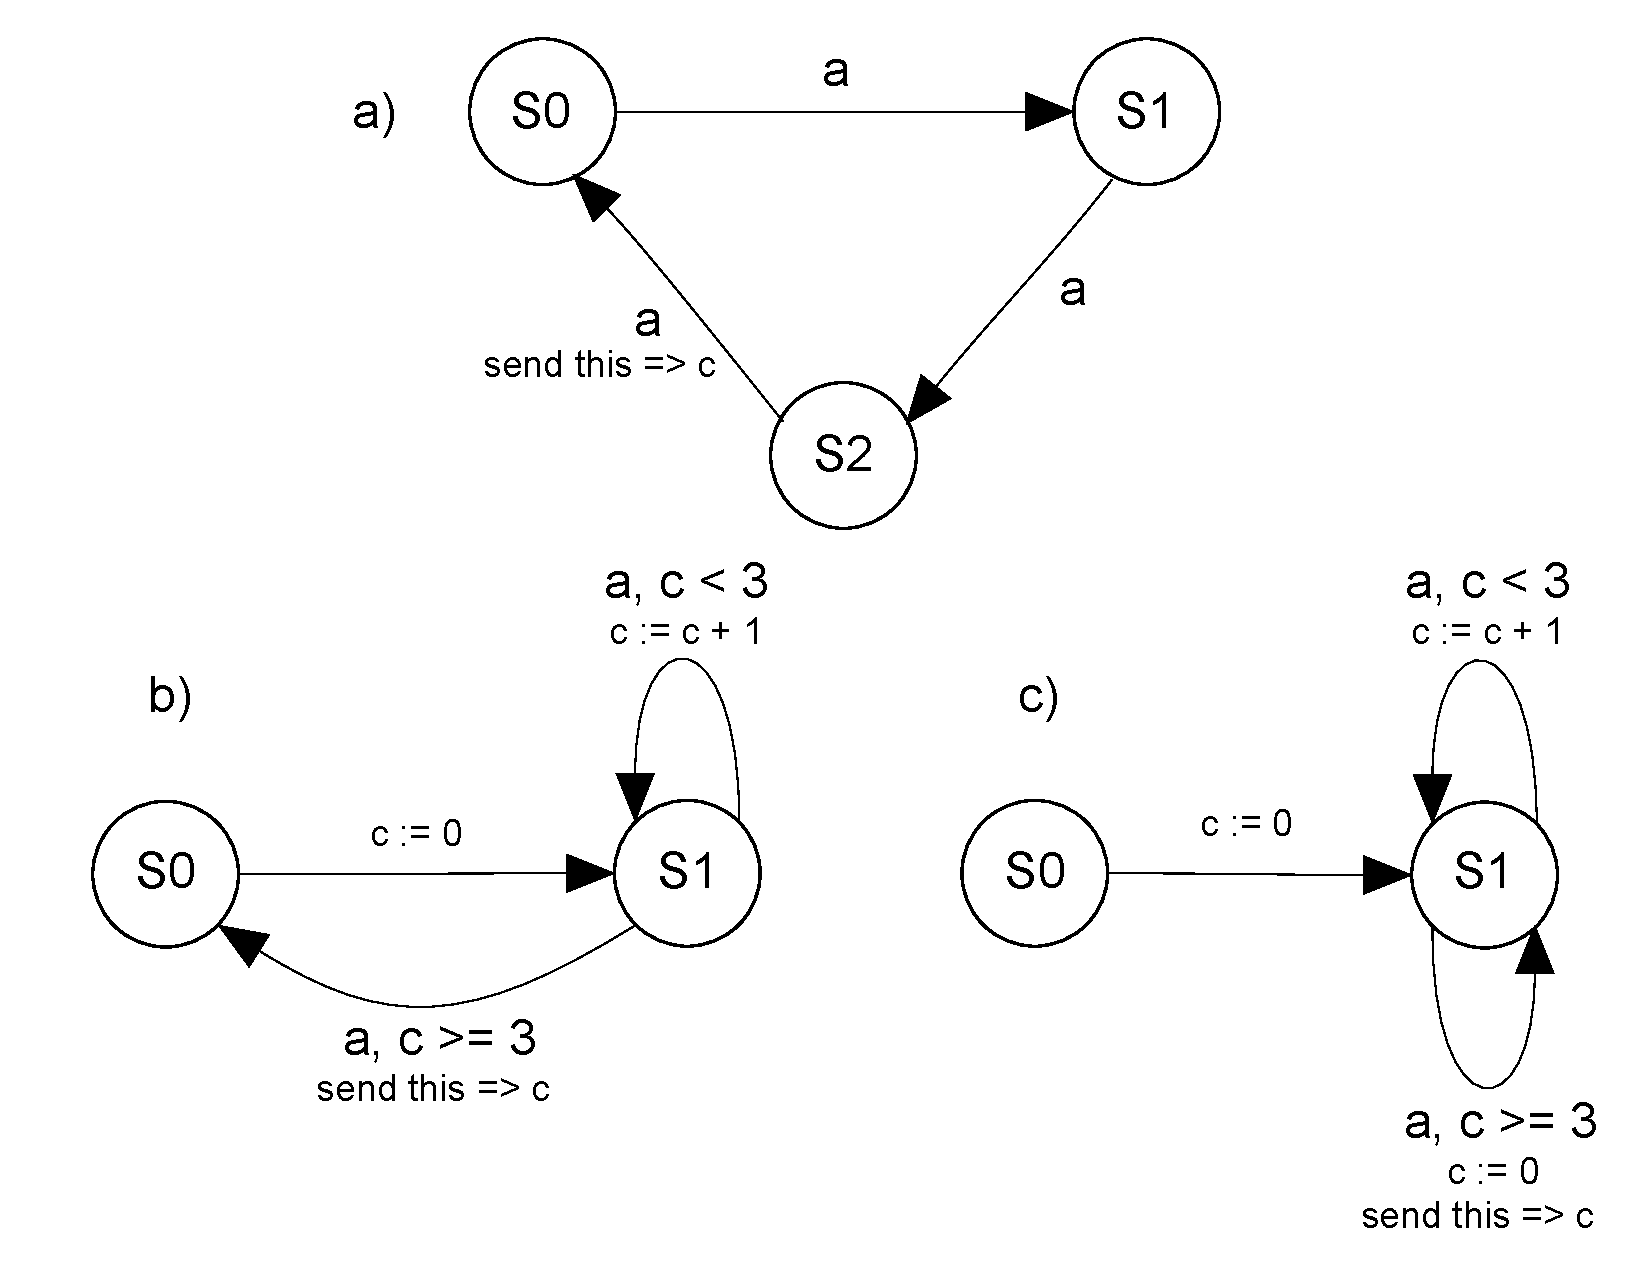
\includegraphics[scale=0.4]{figs/counter.pdf}
  \caption{The transition diagrams of the counter synchroniser.}
  \label{fig:counter}
  \end{figure}


  \item The selection predicate $\rho$

In a given state $k$ for each output channel $\omega_{m}$ we note all $i$ on which $\rho_{ki}^{m}$ is true. Those message values must be stored in a previous state and recalled in state $k$. It is expected that the boolean vector $\omega_{i} = \rho_{ki}^{m}$ has only very few true elements.

Consequently the storage mechanism that \ak\ provides for synchronisers is in the form of individual \emph{store} variables. The type of a store variable is determined when a variable is assigned.

\textbf{Example: the binary zip synchroniser}  Zip2 receives messages on its input channels and sends their concatenation to the output channel. In the resulting concatenation there's exactly one message from each input channel and those messages are ordered as they received.

The zip2 transition diagram is given in Figure \ref{fig:zip2}. The message received in the current transition is referred by a keyword \emph{this}. $ma$ and $mb$ are the store variables associated with the input channels $a$ and $b$ respectively. The statement \emph{send} indicates a sending of a message to an output channel.

  \begin{figure}[here]
  \centering
  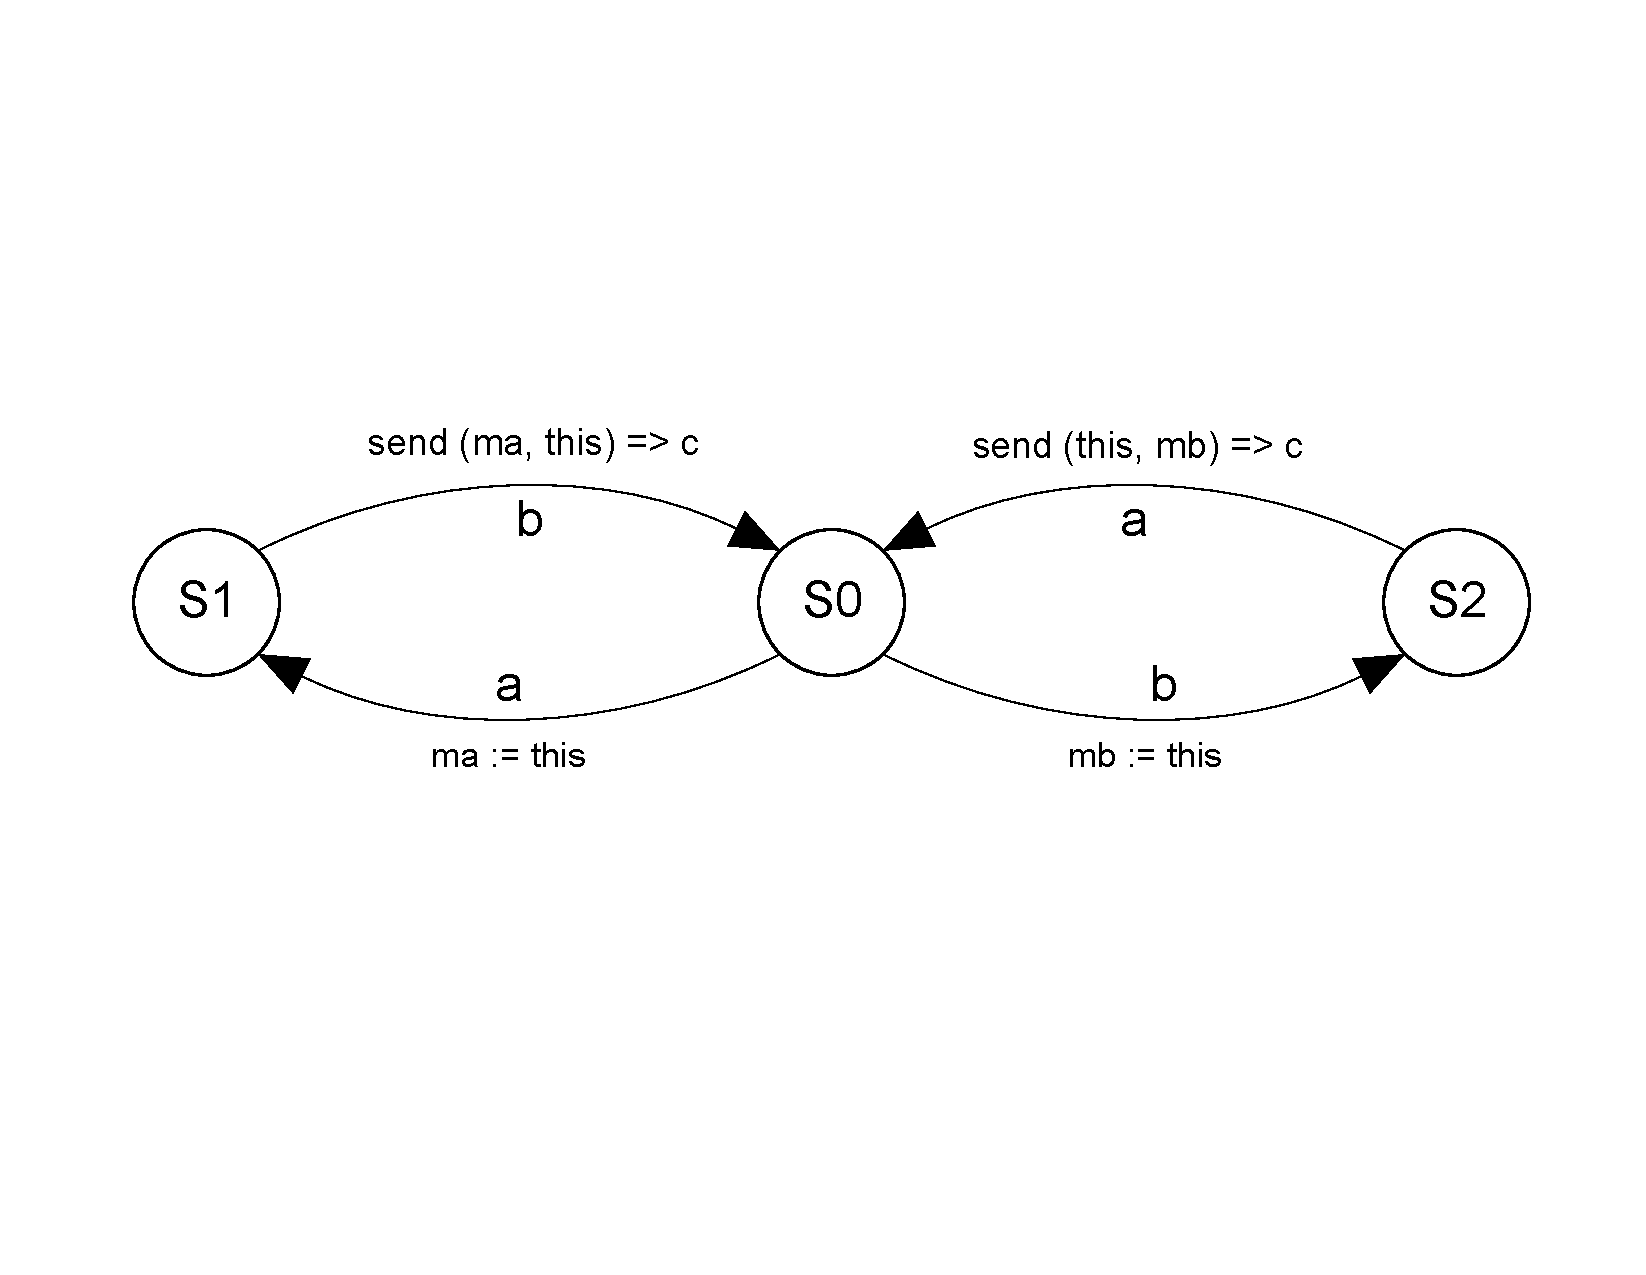
\includegraphics[scale=0.4]{figs/zip2.pdf}
  \caption{The transition diagram of the zip2 synchroniser.}
  \label{fig:zip2}
  \end{figure}

Mathematical model $S_{zip2} = (\Phi, \; \Pi)$, where
  \begin{itemize}
  \item[] $\Phi = (A, \; S, \; T)$,
    \begin{itemize}
    \item[] $C = (a, \; b)$, $P = (true)$, $A = C \times P = ((a, \; true), \: (b, \; true))$,
    \item[] $S = (s_{0}, s_{1}, s_{2})$, $s_{0}$ -- start state,
    \item[] $T$:
      \begin{tabular}{c|c|c|c}
      $A$ \textbackslash $S$ & $s_{0}$ & $s_{1}$ & $s_{2}$\\
      \hline
      $(a, \; true)$ & $s_{1}$ & $s_{1}$ & $s_{0}$\\
      \hline
      $(b, \; true)$ & $s_{2}$ & $s_{0}$ & $s_{2}$\\
      \end{tabular}
    \end{itemize}
  \item[] $\Pi \: : \: S \times \Omega \to V$,
    \begin{itemize}
    \item[] $\Omega = (c)$,
    \item[] $V = ((a, \; b), \: (b, \; a))$
    \end{itemize}
  \end{itemize}

An output message is emitted when a transition happens either from the state $s_{1}$ or the state $s_{2}$. These states are reached in two paths:
  \begin{itemize}
  \item[]
$W_{0} = ((s_{0}, \; a), \: (s_{1}, \; b))$

$\Pi \; (s_{1}, c) = \psi_{\sqcap} \; \{\mu_{0} = a \: | \: \rho_{10}^{c} \; (s_{0}) = 1, \mu_{1} = b \: | \: \rho_{11}^{c} \; (s_{1}) = 1\}$, $k = 1$, $i = 0,1$
  \item[]
$W_{1} = ((s_{0}, \; b), \: (s_{2}, \; a))$

$\Pi \; (s_{2}, c) = \psi_{\sqcap} \; \{\mu_{0} = b \: | \: \rho_{20}^{c} \; (s_{0}) = 1, \mu_{2} = a \: | \: \rho_{22}^{c} \; (s_{2}) = 1\}$, $k = 2$, $i = 0,2$ 
  \end{itemize}
  \end{enumerate}


\section{The language for \ak\ synchroniser}
We develop the language according to chosen message protocol. The protocol restricts anything but a $choice$ termed message trevelling in channels. This the syntax $on a.(x,y, ...)$ is not needed with this protocol. We may include this syntax as a syntax sugar for $uniq$ when choice has just one alternative. Originally this syntax was intended for records in channels. However, the chosen protocal doesn't allow it. For example if we want to extend the protocol for lists to travel in channels, we need to define the union of lists, possibly as a construct with 2 nested lists $(union l_1 l_2)$ and we need to extend the protocol to encode this construct. For record and choice union is easy to define. If no labels in $t_1$ and $t_2$ intersect then the resulting record of choice has all the labels from $t_1$ and $t_2$ with their values: $t = union \; t_1 \: t_2 = union \; {a:t_a} \: {b:t_b} = {a:t_a, \: b:t_b}$. When labels intersect, it is the deal for CAL solver to resolve with option to take (it should consider flow inheritance). The synchroniser just leaves it to be a union of terms:

For example for Choice: $union \; (: \: a:t_a \: :) \: (: \: a:t_b \: :) = (: \: a:union \: t_a, \: t_b \: :)$.
Same for record.


\subsection{Synchroniser code}
%% TODO fix 'channel connected to the port x' to channel x
%% Insert a footer that explains that 'channel x' is short for 'channel connected to the port x'
An \ak\ synchroniser is a finite state machine, therefore the basic building blocks of a synchroniser program are states and transitions. A state of a synchroniser is fully defined by the corresponding state of the finite state machine and the values of the state variables. A transition is the act of moving to another state which is initiated by a triggering event. A triggering event for the synchroniser transition is an arrival of a message to the associated channel. The message may be required to have a specific structure. In addition, a transition may be guarded by special conditions on the values of the state variables. If the conditions are satisfied the transition fires, otherwise it is cancelled.

Once a transition is known to fire, optional actions may be performed before the underlying state machine makes the move. These actions include changing the state and store variable values and sending messages to the output channels. In order to change the state and store variables, the synchroniser language provides state and store expressions over them.

This section gives an overview of the \ak\ synchroniser programming language. The formal grammar of the \ak\ synchroniser is provided in Appendix \ref{sync_syntax}.

  \subsubsection{Program structure}
A synchroniser program consists of a header followed by the synchroniser's body wrapped in braces. The begining of a synchroniser program is indicated by the keyword $synch$.

The header of a synchroniser program contains the synchroniser's name and the channel signature. The name is an ASCII string that follows the C convention.

The body of the synchroniser lists the state and store variables declarations and the states of the underlying finite state machine. Each state is defined by a list of transitions. Each transition lists its triggering condition which includes an optional guarding state expression, an optional list of actions, and, finally, the destination state.

%  \subsection{Macros}
%%%
%%% We removed macros from the language. The compiler must invoke a preprocessor to expand them.
%%%
%The synchroniser language provides macros to avoid having to trivially alter synchroniser programs. Macros are specified in brackets between the synchroniser's name and its channel signature. An example of a configurable synchroniser can be found in \cite{astrakahn}.

  \subsubsection{Channel signature}
The channel signature defines the input channels and the output channels of the synchroniser and their bracketing depths. The synchroniser header (Fig. \ref{min_sync_head}) declares the synchroniser $min$ with two input channels that are connected to the ports $a$, $b$ and two output channels that are connected to the ports $c$, $d$. If the bracketing depths of the channels are not specified, they are assumed to be 0. Thus, the bracketing depth of the channel $a$ is 0.

The input channel depth $-1$ indicates that the input channel is ignored in the synchroniser program. The output channel with the depth $-1$ must not have data sent to them.

\begin{figure}[h!]
\begin{lstlisting}[frame=single]
synch min (a, b:p | c:2, d:p+1)
\end{lstlisting}
\caption{The synchroniser header}
\label{min_sync_head}
\end{figure}

%% TODO remove read-only state variables

The \ak\ synchroniser allows to declare constant and configurable integer depths for the input and output channels. In addition, the depth of the output channel can be specified with an integer shift to the configurable input channel depth.

The input channels are required to have the bracketing depths specified in the signature. Thus, the channel connected to the port $a$ of the $min$ synchroniser must have zero bracketing depth. The channel connected to the port $b$ has a configurable bracketing depth $p$. Actual values of configurable bracketing depths of input channels are determined by the \ak\ compiler. %Once defined in the signature, configurable bracketing depths may be used in state expressions. They are interpreted as read-only state variables.

The output channels of a synchroniser are guaranteed to have the bracketing depths specified in the channel signature. Thus, the synchroniser $min$ must send messages to the output channel connected to the port $c$ at the depth 2 and optionally at the depths $0$, $1$. The output channel connected to the port $d$ must have the bracketing depth $p+1$ that is the depth of the input channel connected to the port $b$ shifted by $1$.


%% TODO Move all the type details to the implementation details
%% TODO The width of int type is declared explicitly to reduce the number of potential states of automata.
  \subsubsection{Variable declaration}
%% Add about state and store variables initialisation.
%% state int(8) a, b=1, c=8; // assignes a=0 b=1 c=9
%% enum (a,b,c) foo, bar=a;  // assignes foo=0 bar=a
The beginning of state variables declaration is indicated by the keyword $state$. A state variable may be either a signed integer of the constant width or a C-style enumeration. State and store variables names are user-defined indentifiers. A user-defined identifier is an ASCII string that follows the C convention.

%% TODO Should move width determining to the implementation detail
Line 1 in Fig. \ref{sync_statevar} declares state variables $a$, $b$, $c$ of width 4. Thus, all three variables are declared to have integer values in the range $[-8; 7]$. Generally, a state variable of width $n$ has integer values in the range $[-2^{n-1}; 2^{n-1}-1]$.

The state variable $foo$ that is declared in the line 2 in Fig. \ref{sync_statevar} can only be assigned the values $d$, $e$ and $f$ specified in the enumeration. The enumeration values are defined as constants if type $int$. If the values are not specified explicitly, they are assigned consequtive positive integers starting with 0. The width of the $int$ type is $\lceil \log_{2}{n} \rceil + 1$, where $n$ is the number of values in the enumeration. Thus, the variable $foo$ has integer values $d=0$, $e=1$ and $f=2$ of the width $\lceil \log_{2}{3} \rceil + 1 = 3$. If the values are specified explicitly, the width is determined as $\lceil \log_{2}{(m+1)} \rceil + 1$, where $m$ is the biggest value in the enumeration. For the variable $bar$ declared in line 3 of Fig. \ref{sync_statevar} $m=4$ and the width is $\lceil \log_{2}{(5)} \rceil + 1 = 4$.

Integer state variables and enum values can be mixed freely in state expressions. Enum values are interpreted as read-only integer state variables. % constant integers!

\begin{figure}[h!]
\lstset{numbers=left, numberstyle=\small, stepnumber=1, numbersep=8pt}
\begin{lstlisting}[frame=single]
state int(4) a, b, c;
state enum(d, e, f) foo;
state enum(x = 1, y = 2, z = 4) bar;
store msg_a, msg_b;
\end{lstlisting}
\caption{State and store variables declaration}
\label{sync_statevar}
\end{figure}

Store variables declaration begins with a keyword $store$. Line 4 in Fig. \ref{sync_statevar} declares state variables $msg\_a$ and $msg\_b$. Store variables do not need explicit type specification; their types are determined on the first assignment to the variable.

All the state and store variables are global to all the synchroniser states.


  \subsubsection{States and transitions}
States and transitions of the synchroniser define which channels are read and in what order. Fig. \ref{zip_struc} presents the code of the binary zip synchroniser's state machine. Line 1 declares the start state of the synchroniser. The $on$ clause indicates the beginning of the transitions list. In the start state the zip2 synchroniser acceptes messages from both input channels $a$ and $b$. State and store expressions associated with the transition and the destination state are specified in the braces.

\begin{figure}[h!]
\lstset{numbers=left, numberstyle=\small, stepnumber=1, numbersep=8pt}
\begin{lstlisting}[frame=single]
start {
  on:
    a { goto s1;    }
    b { goto s2;    }
}
s1 {
  on:
    b { goto start; }
}
s2 {
  on:
    a { goto start; }
}
\end{lstlisting}
\caption{State machine of the zip2 synchroniser}
\label{zip_struc}
\end{figure}

When the zip2 synchroniser is in the start state and it receives a message from the channels connected to the port $a$, the underlying state machine makes a transition to the state $s1$. In this state the synchroniser can only receive messages from channel connected to the port $b$ since there's no transition triggered by channel connected to the port $a$ and defined in this state. When the message on channel connected to the port $b$ is received, the state machine makes a transition to the start state. Lines 10-13 define similar behaviour in state $s2$.

%% Change 'scopes'. 'Blocks' probably
The synchroniser language supports top-down prioritised transition scopes. They are indicated with the $elseon$ keyword. A synchroniser in state $foo$ in Fig. \ref{sync_scope} acceptes messages from channels connected to the ports $a$, $b$, $c$ and $d$. When no destination state is specified for a transition, a synchroniser makes the transition to the current state. If all channels are ready at the same time in state $foo$, the synchroniser processes messages from either channel $a$ or $b$ first. When all messages from channels connected to the ports $a$ and $b$ are processed the synchroniser receives messages from channels connected to the port $c$. If there're no messages in channels $a$, $b$ and $c$ the synchroniser receives messages from the channel connected to the port $d$.

\begin{figure}[h!]
\lstset{numbers=left, numberstyle=\small, stepnumber=1, numbersep=8pt}
\begin{lstlisting}[frame=single]
foo {
  on:
    a { }
    b { }
  elseon:
    c { }
  elseon:
    d { }
}
\end{lstlisting}
\caption{Prioritised transition scopes}
\label{sync_scope}
\end{figure}


  \subsubsection{State expressions}
State expression is a combination of integer constants, state variables and operators, which computes and produces an integer value. The interpretation of a state expression follows C rules of precedence and association. State expressions can be assigned to state variables. In assumption that the output channel is infinite a synthetic example in Fig. \ref{sync_state_exp} counts the number of messages received from channel connected to the port $a$ between the arrivals of messages in channel connected to the port $b$. Line 1 declares the 8-bit integer $count$ and initialises it with 0. When a message from channel connected to the port $a$ is received the value of $count$ increases by 1 (line 5).

\begin{figure}[h!]
\lstset{numbers=left, numberstyle=\small, stepnumber=1, numbersep=8pt}
\begin{lstlisting}[frame=single]
state int(8) count = 0;
foo {
  on:
    a {
      set count = [count + 1];
    }
  elseon:
    b {
      set n = [count], count = [0];
      send count:[n] => c;
    }
}
\end{lstlisting}
\caption{Use of state variables and expressions}
\label{sync_state_exp}
\end{figure}

When a message from channel connected to the port $b$ is received the value of $count$ is stored in the temporary variable $n$, set to 0 and then $n$ is sent to the output channel.

The variable $n$ does not have to be declared and is considered alias for the integer expression. Temporary variables are available until the state machine of a synchroniser makes the next move.


  \subsubsection{Triggering of a transition}
The channel name on its own stands for the availability predicate for the corresponding channel, i.e. the condition that a message of any kind is available. Whether a transition takes place depends on the channel status and optionally the content of the messages.

When a message is received on a channel, it can be matched with a pattern in order to extract parameters needed to select a specific transition. Line 3 of Fig. \ref{sync_trans} checks if a message received from the input channel connected to the port $a$ contains label $x$. If it does, the contents of $x$ are stored in a temporary variable $x$. The tail of the message, i.e. everything but the part labeled $x$, is stored in a temporary variable $t$. Both $x$ and $t$ are read-only and available until the state machine makes a move.

TODO: Fix; everything in $.?v(.... \|\| tail)$ before $\|\|$ are integers.
\begin{figure}[h!]
\lstset{numbers=left, numberstyle=\small, stepnumber=1, numbersep=8pt}
\begin{lstlisting}[frame=single]
foo {
  on:
    a.(x || t)  { }
    a.?v        { }
    a.?v(x, y)  { }
    a.@[k]      { }
}
\end{lstlisting}
\caption{Message content extraction}
\label{sync_trans}
\end{figure}

To support message formats where several variants of a message are possible, a qualifier \begin{bf}?\end{bf}$\alpha$ is available as an input condition. It qualifies input messages as belonging to $\alpha$ variant. Line 4 of Fig. \ref{sync_trans} checks if a message received from channel connected to the port $a$ belongs to the variant $v$. Line 5 checks that a message that belongs to the variant $v$ contains only two records labeled $x$ and $y$. 

A channel carries a stream that consists of messages and possibly segmentation marks. In line 6 in Fig. \ref{sync_trans} a message is checked if it is a segmentation mark of the depth $k$. The depth of a segmentation mark can be a state expression.

Several different channels can be tested in any given state, however, once the readiness of a channel was established, the synchroniser is committed. Hence the set of conditions applied to the message on any input channel must be exhaustive. In Fig. \ref{sync_trans} it is not, because there no pattern for messages that do not contain label $x$, do not belong to variant $v$ and are not a segmentation mark of depth $k$ at the same time. In this case the final clause $a$\begin{bf}.else;\end{bf} is assumed. This clause discards the input message and transitions the synchroniser back to its current state.

A transition can be guarded by a state expression. In this case the transition fires only if the guarding expression evaluates to true. The synchroniser in Fig. \ref{sync_g_state_exp} sends every 256-th message to the output channel. Line 1 declares the 8-bit state variable $i$ that is initialised with 0. It is incremented every time a message from channel connected to the port $a$ is received, except when it reaches 255, in which case it is reset 0 and the received message is sent down the channel $c$. 

Values that are matched from the message can be used in guarding state expressions.
\begin{figure}[h!]
\lstset{numbers=left, numberstyle=\small, stepnumber=1, numbersep=8pt}
\begin{lstlisting}[frame=single]
state int(8) i;
start {
  on:
    a & [i < 255] {
      set i = [i + 1];
    }
    a & [i = 255] {
      set i = [0];
      send this => c;
    }
}
\end{lstlisting}
\caption{Use of guarding state expressions}
\label{sync_g_state_exp}
\end{figure}


  \subsubsection{Store expressions and sending messages}
%% TODO Probably fix it after writing about CAL terms.
Store expression is a mechanism to combine data. Data are typed in \ak\. Types are CAL terms. Store expression concatenates data in the user-defined order and therefore results in the data of a valid CAL type. The result of the store expression can be either stored in a store variable or sent down the output channel.

The example in Fig. \ref{sync_send} demonstrates the use of store expressions and the $send$ clause. In the start state the synchroniser receives messages from channel connected to the port $a$ that has label $n$ in it. In line 5 the value under label $n$ is incremented and stored in the store variable $ma$ under label $n$ together with the tail $t$. The syntactic sugar for defining a record is supported. The operator $'$ applied to the variable $x$ creates the record $'x': value(x)$.

%% TODO Provide a more convincing example for 'id and this
\begin{figure}[h!]
\lstset{numbers=left, numberstyle=\small, stepnumber=1, numbersep=8pt}
\begin{lstlisting}[frame=single]
store ma;
start {
  on:
    a.(n || t) {
      set ma = (n:[n+1] || t);
      goto s1;
    }
}
s1 {
  on:
    b {
      send ma || this => c;
      goto start;
    }
}
\end{lstlisting}
\caption{Use of store expressions and the $send$ clause}
\label{sync_send}
\end{figure}

A message received on a channel is referred to by the keyword $this$ within the active transition. In state $s1$ the synchroniser receives messages from channel connected to the port $b$. When a message is received, it is concatenated with the store variable $ma$ (line 12) and sent to the output channel connected to the port $c$.




\section{Execution order of synchroniser\label{execod}}
\begin{itemize}
\item Fairness policy
In a certain state both input channels may be ready, but a state machine receives input symbols one at a time. Which transition will be triggered under such circumstances is defined by the fairness policy: the coordinator will ensure that when more than one transition is possible in a given state, all choices will be made with the same frequency.

\item Non-deterministic $goto$

The purpose of non-deterministic gotos comes from the requirement that the synchroniser must not block the execution. If non-deterministic goto is the case then the synchroniser makes a fair transition to the state that sends messages to the channel that is not blocked.

In other words, the synchoniser avoids to make transitions to the states that send messages to blocked channels.


\item Algorithm of the execution of synchronisers
on-elseon execution order, dead $elseon$ code with $\langle chan \rangle .else$
\end{itemize}


\section{The implementation of the $aksync$ compiler}
The implementation of the compiler is written in Python (TODO: cite a cookbook), with code generation to an intermediate representation that is used by the \ak\ runtime system.

\subsection{Lexical analysis}
  \paragraph{Lexical analyser} PLY
  \paragraph{Preprocessor}
%%%
%%% We removed macros from the language. The compiler must invoke a preprocessor to expand them.
%%%
%The synchroniser language provides macros to avoid having to trivially alter synchroniser programs. Macros are specified in brackets between the synchroniser's name and its channel signature. An example of a configurable synchroniser can be found in \cite{astrakahn}.
Preprocessor performs (a C-like) macro expansion. There's no preprocessor directives in the synchroniser language (like \#define in C). Preprocessor commands are passed to it as a part of the compiler invocation command (a special flag like -Dday=night in C).

With the preprocessor we implement configuration paramenters from the original synchroniser language. Explain why they were removed. Explain what is bad about macros (can substitute anything, even a piece of code).

\subsection{Syntax analysis}
  \paragraph{Syntax alanyser} PLY. Syntax-directed translation. A translation scheme embeds program fragments called semantic actions in production bodies (TODO Dragon book, p.107)

Error handling in PLY.


  \paragraph{Abstract syntax tree} The result of syntax analysis is a representation of the source program called intermediate code. We use abstract syntax tree in the implementation.

TODO: structure of the AST.
AST generator by Eli Bendersky with the reference.

  \paragraph{Symbol table}
Symbol tables are data structures used by compilers to hold information about identifiers in a program's source code. The information is collected incrementally by the analysis phases of a compiler. Entries in the symbol table contain identifier's type, scope level, location and any other relevant information.

The role of a symbol table is to pass information from declarations to uses. A semantic action puts information about identifier $x$ into the symbol table, when the declaration of $x$ is analysed. Subsequenlty, a semantic action associated with a production that involves an identifier gets information about the identifier from the symbol table.

The scope of a declaration is the portion of a program to which the declaration applies. (TODO scope straucture of a sync program). State and store variables are visible for all transitions, therefore they belong to the global scope. State expression aliases and variables that are pattern matched belong to the local scope of a transition.

Symbol tables typically need to support multiple declarations of the same identifier within a program. We shall implement scope by setting up a separate symbol table for each scope (transition) and chaining them. The approach to the implementation of a symbol table is taken from (TODO ref Dragon book, p.89). Chaining of symbol tables results in a tree structure (probably we can simplity it somehow, because we do not really need a tree of scopes).

(TODO: probably a short description of the approach is needed. Class with fields hashtable and a link to the previous scope object, and methods 'create new', 'put', 'get' which searches the chain of tables.)

The symbol table contains types and (possibly) locations. Builing of a symbol table Dragon book p.90.

  \paragraph{Syntax-driven type inference?}
Special language constructs simplify type inference (probably it's not a good word here).

$x$ and $y$ are assigned a special type None.
\begin{figure}[h!]
\begin{lstlisting}
// typeof(x) = None means a term variable
a.?v(x, y || t) {
  // typeof(x) = None
  // typeof(y) = None
  // typeof(this) = DataTyp(h={'x': typeof(x), 'y': typeof(y)}, t='t')
  // typeof(a) = DataTyp(h={'v': typeof(this)}, t='a_tail')

  set n = [x+1], ma = (this || id:y);
  // typeof(x) = IntTyp(None)
  // typeof(n) = IntTyp(None)
  // typeof(ma) = DataTyp(h=typeof(this).h+{'id': typeof(y)}, t='t')

  send (ma || 'n':n) => c;
  // typeof(c) = DataTyp(h=typeof(ma).h+{'n': typeof(n)}, t='t')
}

a.?v(x, y || t) {
  // typeof(x) = None
  // typeof(y) = None
  // typeof(this) = DataTyp(h={'x': typeof(x), 'y': typeof(y)}, t='t')
??  // typeof(a) = DataTyp(h={'v': typeof(this)}, t='a_tail')

  set ma = (this || y);
  // typeof(n) = IntTyp(None)
  // typeof(ma) = DataTyp(h=typeof(this).h+typeof(y).h, t=tailof(this))

  send ?v(ma) => c;
  // typeof(c) = DataTyp(h={'v':typeof(ma)}, t=None)
}




// Remove variant 'v'?
a.?v(x, y || t) {
// typeof(x) = None
// typeof(y) = None
// typeof(this) = DataTyp(h={'x': typeof(x), 'y': typeof(y)}, v='v', t='t')
// typeof(a) = DataTyp(h={'v': typeof(this)}, v=None, t='tail')

set n = [x];
// typeof(x) = IntTyp(width=None)

set m = this || x || 'y || id:z
// typeof(x) = DataTyp(h={'x': None}, v=None, t=None)
// typeof(y), typeof(z) not influenced
// typeof(m) = DataTyp(h=typeof(this).h + {'x': None} + {'y': typeof(y)} + {'id': typeof(z)}, v=None, t=tailof(this))

send this || x || 'y || id:z => c
// typeof(x) = DataTyp(h={'x': None}, v=None, t=None)
// typeof(y), typeof(z) not influenced
// typeof(c) = DataTyp(h=typeof(this).h + typeof(x).h + {'y': typeof(y)} + {'id': typeof(z)}, v=None, t=tailof(this))

send ?v(this || x || 'y || id:z) => c
// typeof(c) = DataTyp(h={'v': typeof(this || x || 'y || id:z)}, v='v', t=None)

\end{lstlisting}
\label{aa}
\end{figure}

If $x$ or $y$ are used in a state expression, their type is assigned to Int.


A state expression is specified in brackets. Everything in state expression is integer.
If an assignment is being parsed and no brackets were specified in assignment expression, then it is a store expression.

  \paragraph{Static checking}
Static checks are consistency checks that are done during compilation. Not only do they assure that a program can be compiled successfully, but they also catch programming errors early. Static checking includes:
\begin{itemize}
\item Syntactic checking. Constraints such as an identifier is declared at most once in a scope (TODO: more)

Reserved words $nil$ and $this$ can't be identifiers

\item Type checking. The type rules of a language assure that an operator or function is applied to the right number and type of operands.

If an identifier was met and it is already in the current scope of symbol table, it must have the same type (int or data) as before.
\end{itemize}

    \paragraph{Tests}
Uses standard python unittest module.
Expands AST into nested list.

\subsection{Semantic analysis}
  \paragraph{Semantic analyser}
Architecture of the analyser. Pattern visitor?

  \paragraph{Checks}
\begin{enumerate}
\item Channel signature. If the output channel depth is in the form of depth expression $p+integer$, then $p$ should be the depth of one of the input channels. $p$ is not allowed anywhere in state expressions.
  \begin{itemize}
  \item (a:p | b:p+1) - allowed
  \item (a:p | b:0) - allowed
  \item (a:p | b:r) - allowed
  \item (a:p | b:r+1) - NOT allowed
  \end{itemize}
The special depth $-1$ indicated that the channel is not used. Therefore, if it is an input channel, all the transitions reading from it can be removed. If it is an output channel, and the transition that sends to this channel is valid, then an error must occur.

!!Probably avoid writing a visitor!! Visitor for ports that returns their depths which are IDs.
For the input and output channels sets that are returned by the visitor are equal.
Do we really need visitor for it?

Check that transitions in states are made on the specified in signature input channels and messages are sent on the specified output channels.

\item State variables.
State variables are in global scope.

int(n) a, b, c; n denotes only the value range of a state variable. It decreases the number of possible states of a synchroniser. $a$, $b$ and $c$ must always be within range $[0; 2^{n}-1]$ (int is unsigned). At low level state variables are machine- and target language- dependent integers.

The translation scheme in Fig. \ref{std} presents state variable types and their ranges.

(Table: grammar rule - type/width, p.375 Dragon book).
\begin{figure}[h!]
\centering
\begin{tabular}{|c|c|}
\hline
Type & Values\\
\hline
int(n) & $[0; 2^{n}-1] \cap \mathbb{Z}$\\
\hline
enum($a_1$, $a_2$, $\dots$ $a_n$) & $[0; n-1] \cap \mathbb{Z}$\\
\hline
enum($a_1=N_1$, $a_2=N_2$, $\dots$ $a_n=N_n$) & $N_1$, $N_2$, $\dots$ $N_n$\\
\hline
\end{tabular}
\caption{Computing types and their value ranges}
\label{std}
\end{figure}

(TODO: Probably it is a static check that can be done right from parser)

Check if the range condition is valid at least for assignments (int(1) x = 10 is not good, should issue a warning, check what would be assigned to x in C). For the state expressions that evaluate during the execution of the synchroniser it's probably ok to delegate the overflow checks to the C compiler.

\item State expressions. Probably it is all static check as well.
  \begin{itemize}
  \item Patterns $(x || t)$ and aliases for state expressions. $x$ and $t$ are in local scope of the active transition.

(TODO: think if it should be restricted). $x$ and $t$ musn't be declared global - otherwise it is an error??

$x$ and $t$ are read-only.

Probably should not differentiate between pattern variables and aliases. For state and store variables there's a differentiation because we need to know what is included in states of synchroniser (state vars) and what is not (store vars).

If $x$ is used in a state expression, it is integer (has the term 'number'). Tail $t$ can't be used in a state expression; $t$ is always at least a record ($t = (name: value)$).

  \item The grammar for integer expression used in our implementation of a synchroniser compiler (Appendix \ref{int_exp_gr}) is a simplified version of the C grammar for arithmetic expression.

  \end{itemize}


\item Store variables
Store variables are typed by CAL terms.
The type of a store variable is determined on the first assignment to it.

\item Store expressions
The result has a valid CAL term.
If the right-hand side of an assignment is not in brackets, it is a store expression.

\end{enumerate}


\subsection{Code optimisation}
  \paragraph{Dead code elimination}
\begin{itemize}
\item Remove unreachable states of an automaton (when there's no state variables involved).

\item Remove unreachable transitions based on Section Execution order.

\item Remove unused state, store variables and assignments (this may require some simple def-use analysis, probably can put it into symbol tables).
\end{itemize}


\subsection{Code generation}
  \paragraph{Synchroniser runtime code}
Give a class diagram?
Generator architecture - node visitor

  \paragraph{Synchroniser passport}
A synchroniser can impose some restriction on the type of messages it accepts.
In the implementation we consider that only choices travel between channels (it is unclear what is a unification of lists, how to order the elements in the resulting list).

None indicates that it is a term variable.

Input channels: Fig. \ref{a}.
\begin{figure}[h!]
\begin{lstlisting}
//term: None (term variable), Int, Record, Choice
a.(x,y||t) {
  //x - is a value not a pair. In a store expression of in a send it must be 'x
  //term(x) = None
  //term(y) = None
  //term(a) = { x:term(x), y:term(y) | $t }
  //term(this) = term(a)

  set n = [x];
  //term(x) = Int
  //term(a) = { x:term(x), y:term(y) | $t }
}

a.?v(x,y||t) {
  //term(x) = None
  //term(y) = None
  //term(this) = { x:term(x), y:term(y) | $t }
  //term(a) = (: v:term(this) | $a_t :)

  set n = [x];
  //term(x) = Int
  //term(a) = (: v:{ x:term(x), y:term(y) | $t } | $a_t :)
}
\end{lstlisting}
\label{a}
\end{figure}

Output channels: Fig. \ref{b}.
\begin{figure}[h!]
\begin{lstlisting}[frame=single]
//record union with label 'x' collision: {x:type_1, y:...} + {x:type_2, z:...} = {x:type_2, y:..., z:...}
//python's dict.update(...)
a.(x,y||t) {
  //term(x) = None
  //term(y) = None
  //term(this) = { x:term(x), y:term(y) | $t }
  //term(a) = term(this)

  set ma = (this || id:y);
  //term(ma) = term(this) || id:term(y) =
             = { x:term(x), y:term(y), id:term(y) | $t }

  send ?v(ma || n:x) => c;
  //term(c) = (: v:(term(ma) || n:x) | $c_t :) =
            = (: v:{ x:term(x), y:term(y), id:{ y:term(x) }, n:term(x) | $t } | $c_t :)
}
\end{lstlisting}
\label{b}
\end{figure}


\section{Discussion}
MDL is wider than what the presented synchroniser can synchronise. TODO: give examples. However, it need to be elaborated with the real world applications of \ak\ whether it is useful to implement it in synchronisers.

Decide how to do flow inheritance in synchronisers. This will be done outside of synchronisers. Need to somehow specify which fields are inherited and which are not. In synchroniser transitions we can pick fields of an accepted message, with ehich we want to do something in synchroniser. However, there may be many fields in the message and some of them do not need to be inherited. In theory we could pick all the fields that we want to inherit along with the fields we want to work with, and them concat them and send them to then output channel. But there may be too many to specify manually for eack transition in the synchroniser caused by the channel.



\bibliographystyle{unsrt}
\bibliography{report}

\end{document}
